% =====================================================================
% TV3: Trần Kim Ngọc
% Phần II: Tương tác như một Generative Model
% Phần III: Học Likelihoods
% Phần IV: Data Tự Sinh
% =====================================================================

% =====================================================================
\section{Phần II: Tương tác như một Generative Model}
% =====================================================================

Trong Phần I, chúng ta đã thấy cách các generative model có thể được
tích hợp vào các thuật toán RL hiện có dưới dạng world model hoặc
policy. Phần II tiến thêm một bước: thay vì chỉ \textit{sử dụng}
generative model trong RL, chúng ta sẽ nhìn nhận bản thân quá trình
tương tác của RL agent với môi trường như một \textbf{quá trình
generative}. Góc nhìn mới này mở ra những thuật toán và ứng dụng
hoàn toàn mới, đặc biệt là khả năng loại bỏ sự phụ thuộc vào reward
function -- một trong những thách thức lớn nhất của RL trong thực tế.

% ---------------------------------------------------------------------
\subsection{RL Agent là Generative Model}
% ---------------------------------------------------------------------

\subsubsection{Generative Model là gì?}

Một generative model thường được hiểu là một mô hình có khả năng:
\begin{enumerate}
    \item \textbf{Tạo ra mẫu} (sampling) từ một phân phối nào đó.
    \item \textbf{Ước lượng likelihood} (khả năng xảy ra) của các mẫu.
\end{enumerate}

Ví dụ quen thuộc bao gồm language model, diffusion model, VAE hay
Gaussian mixture model. Điểm chung của các mô hình mạnh nhất là chúng
đều thực hiện \textbf{tính toán lặp đi lặp lại} để tạo ra mẫu: VAE và
normalizing flow biến đổi một vector nhiễu qua nhiều lớp mạng neural,
diffusion model lặp đi lặp lại quá trình khử nhiễu để tạo ra ảnh chất
lượng cao.

\subsubsection{RL Agent như một Quá trình Generative}

Một RL agent tương tác với môi trường theo chuỗi:
\[
s_0 \xrightarrow{\pi} a_0 \xrightarrow{p} s_1 \xrightarrow{\pi} a_1
\xrightarrow{p} s_2 \xrightarrow{\pi} \cdots
\]

Nếu nhìn từ góc độ generative modeling, quá trình này có thể được coi
là một \textbf{generative model của các quan sát}, trong đó:
\begin{itemize}
    \item \textbf{Mẫu được tạo ra} = quan sát $s_f$ tại một thời điểm
    nào đó trong tương lai.
    \item \textbf{Tính toán lặp lại} = chuỗi tương tác
    policy-environment qua nhiều bước thời gian.
    \item \textbf{Điều kiện hóa} = thông tin bổ sung cung cấp cho
    policy (ví dụ: goal, ngôn ngữ).
\end{itemize}

Hình~\ref{fig:rl_as_genai} minh họa sự tương đồng này: trong khi
diffusion model thực hiện các bước khử nhiễu để tạo ra ảnh đẹp, RL
agent thực hiện các bước tương tác để đến được trạng thái mong muốn.

\begin{figure}[H]
    \centering
    % Trích từ tutorial Eysenbach & Zhang, ICML 2025
    \includegraphics[width=0.8\textwidth]{images/rl_as_genai.png}
    \caption{So sánh giữa generative model thông thường (trái) và RL
    agent (phải). Cả hai đều thực hiện tính toán lặp lại để tạo ra kết
    quả mong muốn. Nguồn: \cite{eysenbach2025tutorial}.}
    \label{fig:rl_as_genai}
\end{figure}

\subsubsection{Tại sao Góc nhìn này Hữu ích?}

Góc nhìn ``RL là Generative AI'' mang lại ba lợi ích quan trọng
\cite{eysenbach2025tutorial}:

\textbf{(1) Ngôn ngữ hình thức cho tương tác.} Hầu hết các LLM hiện
tại thực hiện suy luận thuần túy trong ``tâm trí'' -- không thực sự
thay đổi thế giới. Để AI có thể tương tác với con người, công cụ và
môi trường vật lý, cần một ngôn ngữ hình thức mô tả quá trình tương
tác. RL cung cấp chính xác ngôn ngữ đó. Coi tương tác như một quá
trình generative cho phép tận dụng toàn bộ bộ công cụ của generative
AI để xây dựng các hệ thống có khả năng hành động trong thế giới thực.

\textbf{(2) Giải quyết thách thức thiết kế reward.} Reward engineering
-- thiết kế hàm phần thưởng -- là một trong những thách thức thực tế
lớn nhất của RL. Với bài toán dọn phòng robot, người thiết kế phải tự
hỏi: nhặt một chiếc áo được bao nhiêu điểm? Xếp sách ngay ngắn được
bao nhiêu? Đây là công việc tốn kém và dễ sai. Bằng cách định nghĩa
lại bài toán RL theo hướng goal-reaching (đạt đến trạng thái đích),
chúng ta có thể loại bỏ hoàn toàn nhu cầu thiết kế reward thủ công.

\textbf{(3) Thống nhất với các lĩnh vực ML khác.} Trong học có giám
sát, bài toán được định nghĩa qua dữ liệu. Trong RL truyền thống, bài
toán được định nghĩa qua scalar reward -- một sự bất hòa với phần còn
lại của ML. Góc nhìn generative cho phép định nghĩa bài toán RL qua
dữ liệu (trạng thái đích mong muốn), thống nhất với phương pháp luận
của toàn bộ cộng đồng ML.

% ---------------------------------------------------------------------
\subsection{Goal-Conditioned Reinforcement Learning}
% ---------------------------------------------------------------------

\subsubsection{Định nghĩa Bài toán Goal-Reaching}

Thay vì sử dụng scalar reward, goal-conditioned RL định nghĩa nhiệm vụ
bằng một \textbf{trạng thái đích} $g$ mà agent cần đạt tới. Mục tiêu
được hình thức hóa như sau:

\begin{equation}
    \max_\pi (1-\gamma) \mathbb{E}_\pi \left[ \sum_t \gamma^t
    p(s_{t+1} = g \mid s_t, a_t) \right]
    \label{eq:goal_reaching}
\end{equation}

Phương trình~\eqref{eq:goal_reaching} có thể được hiểu trực quan như
sau: agent nhận phần thưởng +1 khi ở tại goal $g$ và +0 khi không ở
đó, với hệ số chiết khấu $\gamma$ khuyến khích đến goal càng sớm càng
tốt. Việc định nghĩa mục tiêu theo xác suất $p(s_{t+1} = g \mid s_t,
a_t)$ thay vì hàm indicator $\mathbf{1}(s_t = g)$ cho phép hoạt động
tốt trong cả không gian trạng thái liên tục lẫn rời rạc.

Mục tiêu này tương đương với bài toán RL tiêu chuẩn với hàm reward:
\begin{equation}
    r_g(s, a) = (1-\gamma) \, p(s' = g \mid s, a)
    \label{eq:goal_reward}
\end{equation}

Điểm quan trọng của công thức~\eqref{eq:goal_reward} là reward được
định nghĩa trực tiếp qua \textbf{dữ liệu} (trạng thái đích $g$) thay
vì qua các giá trị scalar do người thiết kế quy định.

\subsubsection{Ứng dụng Thực tế}

Goal-reaching có rất nhiều ứng dụng thực tế
\cite{eysenbach2025tutorial}:
\begin{itemize}
    \item \textbf{Robot locomotion và manipulation}: robot học cách di
    chuyển đến vị trí mục tiêu hoặc thao tác đối tượng về trạng thái
    mong muốn.
    \item \textbf{Lái xe tự động}: xe học cách đến đích trong các điều
    kiện giao thông khác nhau.
    \item \textbf{Tổng hợp hóa học}: tìm chuỗi phản ứng để tổng hợp
    phân tử mục tiêu.
    \item \textbf{Games}: xây dựng công trình trong Minecraft, giải câu
    đố.
\end{itemize}

\subsubsection{Goal-Conditioned Behavioral Cloning (GCBC)}

Một phương pháp đơn giản và hiệu quả để học goal-reaching từ dữ liệu
là \textbf{Goal-Conditioned Behavioral Cloning (GCBC)}
\cite{eysenbach2025tutorial}. Thay vì học policy $\pi(a \mid s)$,
GCBC học policy có điều kiện theo goal $\pi_\theta(a \mid s, g)$ bằng
cách tối đa hóa:

\begin{equation}
    \max_\pi \mathbb{E}_{\tau \sim \mathcal{D},\, (s,a,s_f)}
    \left[ \log \pi_\theta(a \mid s,\, g = s_f) \right]
    \label{eq:gcbc}
\end{equation}

Công thức~\eqref{eq:gcbc} có thể được hiểu theo quy tắc Bayes: học
policy tối đa hóa likelihood trên là tương đương với tối đa hóa:

\begin{equation}
    \max_{\pi_\theta} \mathbb{E}_{a \sim \pi_\theta(a|s,g)} \left[
    \log \mathbb{E}\left[\sum_t \gamma^t \mathbf{1}(s_t = g)
    \mid s, a\right] + \log \beta(a \mid s) \right]
    \label{eq:gcbc_bayes}
\end{equation}

trong đó $\beta(a \mid s)$ là behavior policy -- phân phối hành động
trong dữ liệu gốc. Số hạng $\log \beta(a \mid s)$ đóng vai trò
\textbf{regularization}, ngăn policy học các hành động quá khác biệt
so với dữ liệu training.

Một điểm thú vị của GCBC là kỹ thuật \textbf{masking}: mô hình che đi
một số token trạng thái hoặc hành động trong chuỗi và học cách điền
vào chỗ trống (tương tự BERT). Điều này làm mờ ranh giới giữa world
model và policy -- \textit{một generative model duy nhất có thể vừa
dự đoán hành động tiếp theo (vai trò policy) vừa dự đoán trạng thái
tiếp theo (vai trò world model)}, tùy thuộc vào token nào bị che.

% =====================================================================
\section{Phần III: Học Likelihoods}
% =====================================================================

Phần II đã giới thiệu cách nhìn nhận tương tác như một quá trình
generative và sử dụng góc nhìn này cho bài toán goal-reaching. Phần
III mở rộng thêm: nếu tương tác là một generative model, thì chúng ta
có thể \textbf{ước lượng likelihood} của các kết quả quan sát được
không? Câu trả lời là có, và điều này cho phép giải quyết các bài toán
RL tổng quát hơn nhiều so với goal-reaching đơn thuần.

% ---------------------------------------------------------------------
\subsection{Successor Measure và Temporal Contrastive Learning}
% ---------------------------------------------------------------------

\subsubsection{Định nghĩa Successor Measure}

\textbf{Successor measure} (hay discounted state occupancy measure)
$p^\pi(s_f)$ được định nghĩa là xác suất agent đến được trạng thái
$s_f$ tại một thời điểm nào đó trong tương lai:

\begin{equation}
    p^\pi(s_f) \triangleq (1-\gamma) \mathbb{E}_\pi \left[
    \sum_t \gamma^t p(s_{t+1} = s_f \mid s_t, a_t) \right]
    \label{eq:successor_measure}
\end{equation}

Đây chính xác là likelihood của việc ``sampling'' trạng thái $s_f$ từ
generative model được định nghĩa bởi RL agent. Phiên bản có điều kiện
$p^\pi(s_f \mid s, a)$ cho biết xác suất đến $s_f$ khi bắt đầu từ
trạng thái $s$ và thực hiện hành động $a$.

\subsubsection{Ước lượng qua Temporal Contrastive Learning}

Việc ước lượng trực tiếp $p^\pi(s_f)$ trong không gian chiều cao rất
khó khăn. Một hướng tiếp cận hiệu quả hơn là ước lượng
\textbf{tỉ lệ xác suất tương đối}:

\begin{equation}
    \frac{p^\pi(s_f \mid s, a)}{p(s_f)}
    \label{eq:prob_ratio}
\end{equation}

Tỉ lệ này có thể được ước lượng như một bài toán phân loại: phân biệt
các cặp $(s, a, s_f)$ mà $s_f$ thực sự là trạng thái tương lai của
$(s, a)$ (positive examples) với các cặp ngẫu nhiên (negative
examples). Classifier $f_\theta(s, a, s_f)$ được huấn luyện với loss:

\begin{equation}
    \min_\theta \; - \mathbb{E}_{p^\pi(s_f|s,a)p(s,a)}
    \left[ \log \frac{1}{1 + \frac{1}{f_\theta(s,a,s_f)}} \right]
    - \mathbb{E}_{p(s_f)p(s,a)}
    \left[ \log \frac{1}{1 + f_\theta(s,a,s_f)} \right]
    \label{eq:contrastive_loss}
\end{equation}

Tại điểm tối ưu: $f_\theta(s, a, s_f) = \frac{p^\pi(s_f \mid s,
a)}{p(s_f)}$. Đây chính là \textbf{temporal contrastive learning}
\cite{eysenbach2025tutorial}.

\subsubsection{Biểu diễn Tham số hóa}

Thay vì coi $f_\theta$ như một black-box, có thể tham số hóa dưới dạng
tích vô hướng của hai biểu diễn:

\begin{equation}
    f_\theta(s, a, s_f) = e^{F_\theta(s,a)^\top B_\theta(s_f)}
    \label{eq:log_linear}
\end{equation}

trong đó $F_\theta(s, a)$ là \textit{forward representation} của cặp
state-action và $B_\theta(s_f)$ là \textit{backward representation}
của trạng thái đích. Biểu diễn này có nhiều tính chất thú vị:
\begin{itemize}
    \item \textbf{Scaling}: mạng lớn hơn cho kết quả tốt hơn đáng kể,
    lên đến mạng 1000 lớp \cite{eysenbach2025tutorial}.
    \item \textbf{Emergent exploration}: chiến lược khám phá tự xuất
    hiện trong quá trình huấn luyện.
    \item \textbf{Triangle inequality}: biểu diễn học được thỏa mãn
    bất đẳng thức tam giác, cho phép lập kế hoạch qua nội suy.
    \item \textbf{Horizon generalization}: huấn luyện trên task
    horizon ngắn, giải được task horizon dài.
\end{itemize}

Q-function cũng có thể được ước lượng từ các biểu diễn này:
\begin{equation}
    Q(s, a) \approx \frac{1}{k} \sum_{s_f, r} f_\theta(s, a, s_f)
    \cdot r(s_f)
    \label{eq:q_from_repr}
\end{equation}

Điều này cho thấy một reward function bất kỳ có thể được biểu diễn
như một vector $z$ duy nhất -- nền tảng cho zero-shot RL.

% ---------------------------------------------------------------------
\subsection{RLZero: Zero-shot RL từ Ngôn ngữ Tự nhiên}
% ---------------------------------------------------------------------

\subsubsection{Vấn đề và Động lực}

Dù các phương pháp zero-shot RL đã cho phép suy ra policy tối ưu cho
bất kỳ reward function nào, việc \textit{chỉ định} reward function vẫn
là thách thức. Ngôn ngữ tự nhiên là kênh giao tiếp trực quan nhất
giữa con người và AI, nhưng các phương pháp trước đây yêu cầu:
\begin{itemize}
    \item Dữ liệu có nhãn liên kết ngôn ngữ với hành vi trong domain
    cụ thể.
    \item Huấn luyện thêm khi nhận lệnh mới.
\end{itemize}

\textbf{RLZero} \cite{sikchi2025rlzero} giải quyết cả hai vấn đề trên,
cho phép suy ra policy trực tiếp từ câu lệnh ngôn ngữ \textbf{mà không
cần bất kỳ supervision trong domain nào}.

\subsubsection{Framework: Imagine -- Project -- Imitate}

RLZero gồm ba bước chính, minh họa trong Hình~\ref{fig:rlzero}:

\begin{figure}[H]
    \centering
    % Trích từ Sikchi et al., NeurIPS 2025
    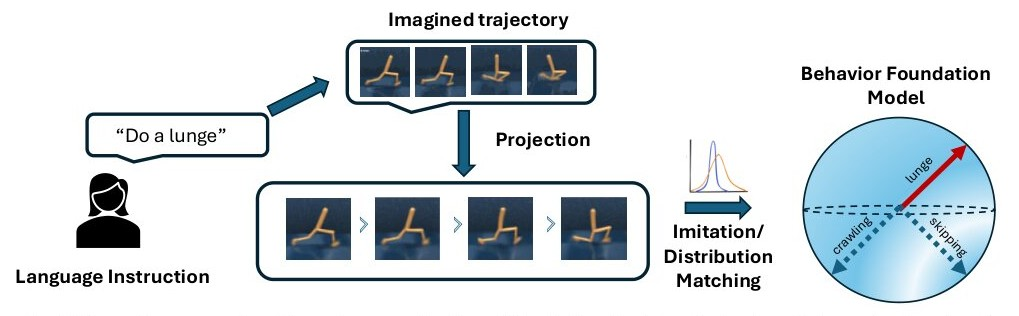
\includegraphics[width=0.85\textwidth]{images/rlzero_framework.png}
    \caption{Framework của RLZero gồm 3 bước: Imagine (tưởng tượng
    video từ ngôn ngữ), Project (chiếu về không gian quan sát của
    agent), Imitate (suy ra policy zero-shot). Nguồn:
    \cite{sikchi2025rlzero}.}
    \label{fig:rlzero}
\end{figure}

\textbf{Bước 1 -- Imagine (Tưởng tượng):}

Cho câu lệnh ngôn ngữ $\ell$ (ví dụ: ``Do a lunge''), Video Foundation
Model VM sinh ra chuỗi frame video $\{i_1, i_2, \ldots, i_T\}$ thể
hiện hành vi tương ứng:
\[
\text{VM}(f_l(\ell)) = (i_1, i_2, \ldots, i_T)
\]
Video model được huấn luyện hoàn toàn không có nhãn (unsupervised)
trên dữ liệu tương tác offline của agent, sử dụng InternVideo2 làm
video-language encoder và kiến trúc GRU đơn giản cho việc sinh video.

\textbf{Bước 2 -- Project (Chiếu):}

Video được tưởng tượng có thể không khớp với domain của agent (khác
embodiment, background, physics). Bước Project sử dụng
\textbf{semantic similarity} để tìm frame thực tế trong dataset gần
nhất với mỗi frame tưởng tượng:

\begin{equation}
    o_t = \arg\max_{o_t} \frac{\mathcal{E}(o_{t-k:t}) \cdot
    \mathcal{E}(i_{t-k:t})}{\|\mathcal{E}(o_{t-k:t})\|
    \|\mathcal{E}(i_{t-k:t})\|}
    \quad \forall t \in [T]
    \label{eq:projection}
\end{equation}

trong đó $\mathcal{E}$ là hàm embedding của SigLIP -- một mô hình
vision-language được pretrain trên dữ liệu internet-scale. Sử dụng
$k=3$ frame liên tiếp giúp nắm bắt thông tin về vận tốc và gia tốc,
cải thiện độ chính xác matching.

\textbf{Bước 3 -- Imitate (Bắt chước):}

Đây là bước cốt lõi của RLZero. Cho chuỗi trạng thái projected
$\{s_1, s_2, \ldots, s_T\}$ như ``expert trajectory'', bài toán
imitation learning được công thức hóa như distribution matching:

\begin{equation}
    z_{\text{imit}} = \arg\min_z \mathcal{D}(\rho^{\pi_z}(s),
    \rho^E(s))
    \label{eq:imitation}
\end{equation}

trong đó $\rho^E$ là phân phối trạng thái của expert trajectory và
$\rho^{\pi_z}$ là phân phối trạng thái của policy $\pi_z$.

\textbf{Theorem 1} \cite{sikchi2025rlzero} chứng minh rằng với KL
divergence, $z_{\text{imit}}$ có thể tính được dưới dạng closed-form
mà \textit{không cần gradient updates hay tương tác với môi trường}:

\begin{equation}
    z_{\text{imit}} = \mathbb{E}_{\rho^E}[\phi(s)]
    \label{eq:zimit}
\end{equation}

trong đó $\phi(s)$ là backward representation đã học của BFM. Nói cách
khác, $z_{\text{imit}}$ chỉ đơn giản là \textbf{trung bình của các
state representations trong expert trajectory} -- một phép tính cực
kỳ đơn giản và hiệu quả.

\subsubsection{Kết quả Thực nghiệm}

RLZero được đánh giá trên 25 tasks trong 4 môi trường continuous
control từ DeepMind Control Suite: Walker, Cheetah, Quadruped, và
Stickman. Kết quả (Bảng~\ref{tab:rlzero_results}) cho thấy:

\begin{table}[H]
    \centering
    \caption{Win rate của các phương pháp khi so sánh với baseline
    TD3+Image-language reward. Nguồn: \cite{sikchi2025rlzero}.}
    \label{tab:rlzero_results}
    \begin{tabular}{lcc}
        \toprule
        \textbf{Phương pháp} & \textbf{Win Rate} &
        \textbf{Thời gian Inference} \\
        \midrule
        Image-language reward (IQL)  & 51.2\% & Vài giờ \\
        Video-language reward (TD3)  & 40.0\% & Vài giờ \\
        GenRL                        & 76.8\% & 3--5 giờ/task \\
        \textbf{RLZero (của chúng tôi)} & \textbf{83.2\%} &
        \textbf{$\approx$25 giây} \\
        \bottomrule
    \end{tabular}
\end{table}

RLZero đạt win rate \textbf{83.2\%} so với baseline tốt nhất (GenRL:
76.8\%), đồng thời chỉ cần \textbf{khoảng 25 giây} để tạo ra policy
-- nhanh hơn GenRL tới hàng trăm lần (3--5 giờ training).

\subsubsection{Cross-Embodiment Transfer}

Một khả năng đặc biệt của RLZero là \textbf{cross-embodiment
transfer}: có thể bỏ qua bước Imagine và trực tiếp dùng video từ
YouTube (quay người thật) làm expert trajectory cho robot có hình dạng
khác hoàn toàn. RLZero đạt win rate 80\% và 100\% lần lượt trên môi
trường Stickman (2D Humanoid) và HumEnv (3D Humanoid) khi imitating
video người thật -- điều mà chưa phương pháp nào trước đó làm được
\cite{sikchi2025rlzero}.

% =====================================================================
\section{Phần IV: Data Tự Sinh}
% =====================================================================

Trong các phần trước, dữ liệu luôn được coi là cho trước. Phần IV đặt
câu hỏi: làm thế nào để agent \textit{tự thu thập} dữ liệu của mình?
Đây là một câu hỏi quan trọng mà các generative model thông thường
không giải quyết được, nhưng RL lại có bộ công cụ phù hợp.

% ---------------------------------------------------------------------
\subsection{Bài toán Exploration}
% ---------------------------------------------------------------------

Cách phổ biến nhất để nghĩ về exploration là theo nghĩa
\textbf{coverage} -- agent cần khám phá càng nhiều trạng thái càng
tốt. Sử dụng lens của occupancy measures, mục tiêu này có thể được
hình thức hóa: thay vì học occupancy measure gán xác suất cao cho
các trajectory có reward cao (như trong RL thông thường), chúng ta
muốn học occupancy measure gán xác suất cho \textbf{tất cả} các
trajectory:

\[
\text{RL thông thường: } \rho^\pi(s) \text{ tập trung vào vùng
reward cao}
\]
\[
\text{Exploration: } \rho^\pi(s) \text{ trải đều khắp không gian
trạng thái}
\]

Tuy nhiên, exploration không chỉ là đi khắp nơi -- mà còn là
\textbf{chuẩn bị để giải quyết các nhiệm vụ mới trong tương lai}. Câu
hỏi đặt ra là: làm thế nào để agent học các kỹ năng có thể tái sử
dụng từ quá trình khám phá?

% ---------------------------------------------------------------------
\subsection{Empowerment}
% ---------------------------------------------------------------------

\textbf{Empowerment} \cite{eysenbach2025tutorial} là một framework để
định lượng ``khả năng làm nhiều thứ'' của agent tại một trạng thái
nhất định. Empowerment được đo bằng mutual information giữa hành động
và trạng thái tương lai:

\begin{equation}
    I(a; s' \mid s) = \mathcal{H}[s' \mid s] - \mathcal{H}[s' \mid
    s, a] = \mathcal{H}[a \mid s] - \mathcal{H}[a \mid s, s']
    \label{eq:empowerment}
\end{equation}

Trong đó $\mathcal{H}[\cdot]$ ký hiệu entropy. Phương
trình~\eqref{eq:empowerment} có thể được hiểu theo hai cách tương
đương:

\begin{itemize}
    \item \textit{Góc nhìn 1}: Mức độ hành động $a$ làm giảm sự không
    chắc chắn về $s'$ -- tức là hành động tác động đến tương lai mạnh
    đến mức nào.
    \item \textit{Góc nhìn 2}: Mức độ biết trạng thái đích $s'$ cho
    phép suy ra hành động đã thực hiện.
\end{itemize}

Empowerment cao tương ứng với việc agent đứng ở vị trí có
\textit{nhiều lựa chọn}: đứng ở ngã tư có empowerment cao hơn đứng ở
ngõ cụt. Agent học cách tự điều hướng đến các vị trí có empowerment
cao, tích lũy khả năng hành động cho tương lai. Khái niệm này cũng
được mở rộng sang setting \textbf{multi-agent}: thay vì tự empowerment
bản thân, AI agent có thể học cách empowerment con người, hỗ trợ con
người có nhiều lựa chọn và khả năng hành động hơn.

% ---------------------------------------------------------------------
\subsection{Skill Learning}
% ---------------------------------------------------------------------

\subsubsection{Mục tiêu}

Pure exploration hay empowerment maximization đơn thuần không đủ để
trang bị cho agent các kỹ năng cụ thể. Giải pháp là học
\textbf{skills} -- các temporal abstraction có thể tái sử dụng để
giải quyết downstream tasks. Đây còn được gọi là
\textbf{self-supervised reinforcement learning}: agent tự tạo ra reward
của mình thông qua intrinsic motivation.

Mục tiêu toán học là tối đa hóa \textbf{mutual information} giữa skill
label $z$ và trajectory $\tau$:

\begin{equation}
    \max_\pi I^\pi(z; \tau) = \max_\pi \left[ \mathcal{H}[\tau] -
    \mathcal{H}[\tau \mid z] \right]
    \label{eq:skill_mi}
\end{equation}

Phương trình~\eqref{eq:skill_mi} gồm hai số hạng với ý nghĩa đối lập:
\begin{itemize}
    \item $\mathcal{H}[\tau]$: entropy biên của trajectory -- muốn
    \textbf{tối đa hóa}, tức là tổng thể hành vi phải đa dạng (mỗi
    skill làm một hành vi khác nhau).
    \item $\mathcal{H}[\tau \mid z]$: entropy có điều kiện của
    trajectory khi biết skill -- muốn \textbf{tối thiểu hóa}, tức là
    với mỗi skill $z$ cụ thể, hành vi phải nhất quán và dễ đoán.
\end{itemize}

\subsubsection{Thuật toán Thực tế}

Để tối đa hóa~\eqref{eq:skill_mi}, cần có một classifier $q(z \mid s)$
đoán skill từ trạng thái. Thuật toán alternates giữa hai bước:

\textbf{Policy optimization:} với classifier $q$ cố định, bài toán
tương đương RL với reward:
\begin{equation}
    r_t = \log q(z \mid s_t)
    \label{eq:skill_reward}
\end{equation}
Reward cao khi classifier đoán đúng skill từ trạng thái hiện tại --
khuyến khích policy làm hành vi rõ ràng, dễ nhận biết.

\textbf{Posterior optimization:} với policy $\pi$ cố định, cập nhật
$q(z \mid s)$ bằng maximum likelihood trên dữ liệu $(s, z)$.

\subsubsection{Giải quyết Downstream Tasks}

Sau khi học xong tập skills, có nhiều cách sử dụng để giải quyết
downstream tasks:
\begin{enumerate}
    \item \textbf{Enumeration}: liệt kê tất cả skills và chọn skill
    có reward cao nhất.
    \item \textbf{Posterior inference}: dùng $q(z \mid \tau)$ để suy
    ra skill phù hợp từ trajectory mẫu.
    \item \textbf{Hierarchical RL}: coi skills là high-level actions,
    xây dựng MDP mới với horizon ngắn hơn.
\end{enumerate}

\subsubsection{Góc nhìn Nén (Compression)}

Một cách nhìn tổng quát về skill learning là qua lăng kính
\textbf{nén thông tin}:
\begin{itemize}
    \item Học có giám sát: nén $Y$ cho $X$ (labels cho inputs).
    \item Học không giám sát (VAE, LLM): nén tập dữ liệu $X$.
    \item \textbf{Self-supervised RL}: nén một \textbf{MDP} -- không
    phải dữ liệu có sẵn, mà là toàn bộ không gian hành vi của môi
    trường.
\end{itemize}

Sản phẩm của quá trình nén này là một \textbf{Behavioral Foundation
Model (BFM)} -- một policy có thể được ``prompt'' để thực hiện nhiều
hành vi khác nhau, tương tự như cách LLM được prompt để thực hiện
nhiều tác vụ ngôn ngữ. Điểm khác biệt quan trọng: trong khi LLM được
huấn luyện trên dữ liệu curated từ internet, BFM được huấn luyện trên
\textbf{dữ liệu tự thu thập} -- agent tự khám phá môi trường và tự
tạo ra dataset của mình.

% =====================================================================
% PHẦN BONUS: PHÂN TÍCH SÂU HẠN CHẾ VÀ ĐỀ XUẤT CẢI TIẾN
% (Nhằm lấy điểm bonus +1 theo rubric thầy)
% =====================================================================

\subsection*{Phân tích Hạn chế và Đề xuất Cải tiến}
\addcontentsline{toc}{subsection}{Phân tích Hạn chế và Đề xuất Cải tiến}

Trong quá trình nghiên cứu RLZero và các phương pháp liên quan, nhóm
chúng tôi nhận thấy một số hạn chế quan trọng mà bài báo gốc chưa
giải quyết triệt để.

\textbf{Hạn chế 1: ``What I Cannot Imagine, I Cannot Imitate''}

Video generation model được sử dụng trong RLZero có kích thước khá
nhỏ (khoảng 43 triệu tham số) và nhạy cảm với prompt engineering. Khi
gặp các hành vi phức tạp (ví dụ: ``raise hand while standing in
place''), model tưởng tượng sai hoàn toàn (Hình 4a trong
\cite{sikchi2025rlzero}). Đây là một \textbf{bottleneck cơ bản}: chất
lượng của toàn bộ pipeline phụ thuộc hoàn toàn vào khả năng tưởng
tượng của video generation model.

\textit{Phân tích sâu:} Vấn đề này không chỉ đến từ kích thước model
mà còn từ \textbf{distribution mismatch}: video generation model được
huấn luyện trên dữ liệu domain của agent (ví dụ: Stickman animations),
nhưng các hành vi phức tạp có thể nằm ngoài phân phối training. Thêm
vào đó, model sử dụng kiến trúc GRU đơn giản không đủ khả năng mô hình
hóa các hành vi có cấu trúc thời gian dài.

\textit{Hướng cải tiến:} Sử dụng các video foundation model lớn hơn
như Sora hay Stable Video Diffusion, hoặc áp dụng kỹ thuật
\textbf{retrieval-augmented generation}: thay vì sinh video từ đầu,
truy xuất video gần nhất từ một database lớn và dùng làm khởi điểm.

\textbf{Hạn chế 2: Thất bại trong Semantic Search}

Bước Project dựa hoàn toàn vào cosine similarity trong embedding space
của SigLIP. Tuy nhiên, có hai trường hợp thất bại hệ thống:

\begin{enumerate}
    \item \textbf{Background distractors}: SigLIP latches vào đặc
    trưng background (màu sắc, texture) thay vì pose của agent, dẫn
    đến matching sai.
    \item \textbf{Rough symmetries}: với các agent gần đối xứng (Walker
    khi đầu và chân trông gần giống nhau), image retrieval trả về
    frame bị lật ngược hoặc nhầm chiều.
\end{enumerate}

\textit{Phân tích sâu:} Đây là hạn chế \textbf{cơ bản của
representation learning}: SigLIP không được thiết kế đặc biệt cho
việc phân biệt pose của agent trong RL environments. Embedding space
tối ưu cho image-text matching trên internet data không nhất thiết tối
ưu cho body pose matching.

\textit{Hướng cải tiến:} Có thể fine-tune SigLIP trên dữ liệu domain
cụ thể của agent (body pose matching), hoặc sử dụng các representation
chuyên biệt hơn như pose estimation model kết hợp với keypoint
matching. Một hướng khác là học \textbf{domain-adaptive embedding}:
trong bước Project, học thêm một hàm mapping từ video frame về agent
observation space thay vì chỉ dùng cosine similarity trong
general-purpose embedding space.